%!TEX root = informe.tex
\chapter{Análisis de Ciclo de Vida de un adoquín: evaluación del impacto ambiental (EICV)}

\section{Introducción}
La norma UNE–EN-ISO 14040:2006 indica que ``la fase de EICV es para conocer y evaluar la magnitud y cuán significativos son los impactos potenciales ambientales de un sistema del producto a través de todo el ciclo de vida del producto''.

En esta etapa, se utilizan los datos recopilados en la fase de Inventario ICV vistos en el capítulo \ref{cap:inventario} y se hace un enfoque relativo del impacto ambiental basado en la Unidad Funcional, convirtiendo los datos del ICV a unidades comunes, sumando posteriormente los resultados obtenidos dentro de la misma categoría de impacto, siguiendo la metodología explicada en la sección \ref{sec:metodologiaeicv}.

En este proyecto también se desarrollarán las etapas opcionales de normalización, agrupación y ponderación de los resultados.

Como se ha establecido la sección \ref{sec:categoriasimpactoseleccionadas}, para la elección de las categorías de impacto, el método ReCiPe recoge 21 categorías, de las cuales se ha seleccionado las más significativas mediante una previsualización de los resultados:

\begin{itemize}
  \item Cambio climático (CC).
  \item Toxicidad humana (HT).
  \item Formación de partículas (PMF).
  \item Transformación natural de la tierra (NLT).
  \item Agotamiento de metales (MD).
  \item Agotamiento de recursos fósiles (FD)
\end{itemize}

Una vez introducidos los datos del inventario para todas las fases del ciclo de vida del producto en el software de análisis SimaPro, se aplica el método de análisis \textit{ReCiPe Endpoint (H) V1.06 / Europe ReCipe H/A}, previamente explicado en la sección \ref{sec:recipe}.

\section{Evaluación del Impacto Ambiental de la fase de extracción de materias primas, fabricación e instalación}

La red de la fase de extracción de materias primas, fabricación e instalación de la figura \ref{fig:fabric_red} se muestran todos los procesos interrelacionados para dar una perspectiva general de la fase.

\begin{figure}[!htb]
\centering
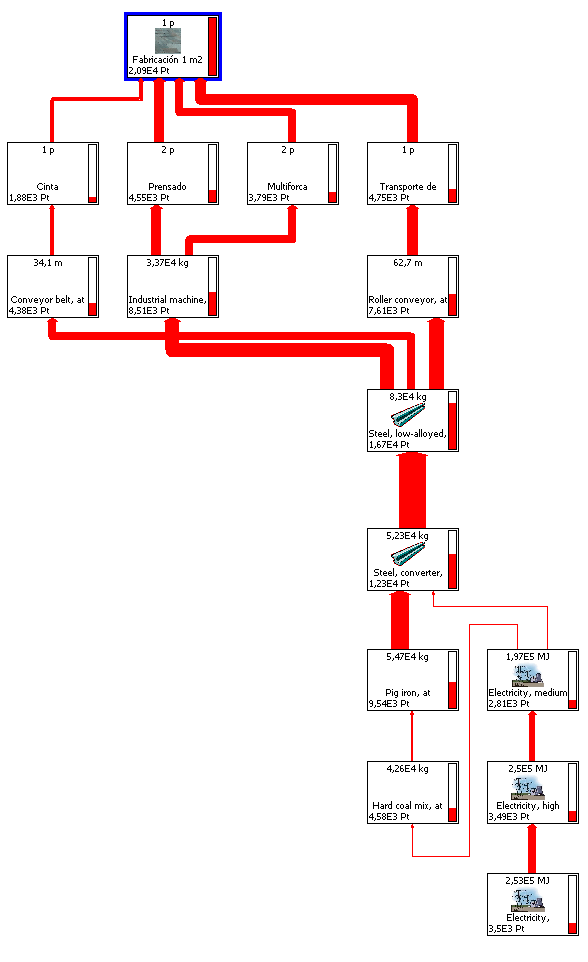
\includegraphics[height=15cm]{img/fabric_red.png}
\caption{Red de la fase de extracción de materias primas, fabricación e instalación.}
\label{fig:fabric_red}
\end{figure}

Cada caja gris representa un proceso y cada proceso se muestra una única vez. Las cajas azul de color azul representan ensamblajes. Las flechas representan los flujos entre procesos. Las barras rojas o termómetros indican la carga medioambiental generada en cada proceso y sus procesos aguas arriba. De esta manera se puede distinguir entre los procesos más importantes y los menos, identificando los puntos calientes.

De la red de la fase de extracción de materias primas, fabricación e instalación se puede deducir que el acero (\textit{Steel, low-alloyed, at plant}) usado por los transportadores de rodillo, cintas transportadoras, prensas y multiforcas es el proceso con mayor carga medioambiental de esta fase.

La caracterización del análisis de impacto muestra todas las categorías de impacto. Cada una de ellas tiene una unidad de medida diferente, por lo que se representan gráficamente de forma porcentual. Para tener una visión más clara de los impactos relevantes de la fase, es mejor recurrir a la normalización donde las diferentes puntuaciones de los impactos caracterizados se relativizan a una referencia común.

La figura \ref{fig:fabric_normalizacion} muestra las categorías de impacto relevantes de esta fase.

\begin{figure}[!htb]
\centering
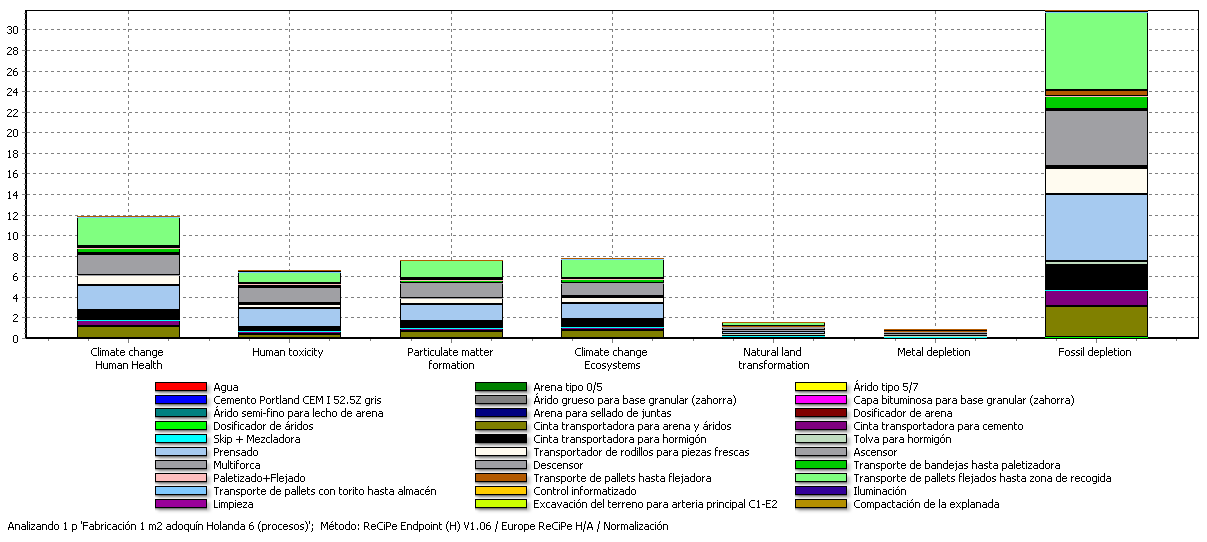
\includegraphics[width=15cm]{img/fabric_normalizacion.png}
\caption{Cuantificación de los impactos normalizados de la fase de extracción de materias primas, fabricación e instalación.}
\label{fig:fabric_normalizacion}
\end{figure}

